Ce travail s'est déroulé en deux principales phases :
Une étape de developement durant laquelle des données et la fonction à apprendre ont été générées.
Et une étape plus appliquée durant laquelle une base de données réelle a été étudiée.\\


Afin d'implémenter informatiquement les concepts théoriques vus précédement,
il a été choistit d'utiliser la librairie Keras\cite{keras}, une reference en python pour faire du machine learning.
La partie sur les intégrales de Choquet a été entièrement recodée en python
avec la librairie numpy\cite{numpy} pour optimiser le temps de calcul.
L'ensembe du code est disponible gratuitement et sous licence libre sur github\cite{repoStage}.

\section{Keras}\label{sec:keras}
La librairie \textsc{Keras} est une interface Python/TensorFlow\cite{tf} permettant de manipuler des réseaux de neurones.
Ici, seul les fonctionnalités principales seront étudiées,
à savoir
création d'un réseau simple,
régression par \sgd\
et évaluation de performances.\\


Voici un exemple de réseau de neurone simple (\textsc{Figure}\ \ref{fig:net2})
qui va tenter d'apprendre l'application linéaire suivante : $f(X) = W\cdot X$.
Avec :
\begin{itemize}
    \item[\textbf{$X$ :}] le vecteur d'entrée tel que : $\dim(X) = 2$.
    \item[\textbf{$W$ :}] le vecteur de poids tel que : $w_1 = 0.2$ et $w_2 = 0.8$.
\end{itemize}
\begin{figure}[H]
    \center
    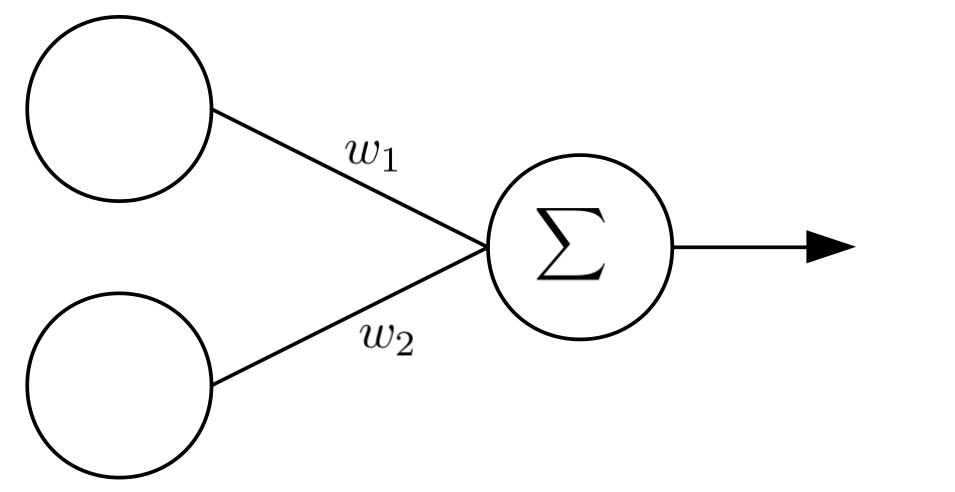
\includegraphics[height=\moyen]{pict/net2.png}
	\caption{Réseau simple}
    \vspace{-10pt}
    \begin{center}
        \footnotesize
        \textit{
        Avec $w_1 = 0.2$ et $w_2 = 0.8$.
        }
    \end{center}
	\label{fig:net2}
\end{figure}
\vspace{-12pt}


Pour créer ce réseau et lui faire apprendre la fonction précédemment citée,
le code suivant est nécessaire :
\newpage
\lstinputlisting[language=Python]{code/reseau1.py}


En exécutant ce code une fois, le résultat suivant est obtenu :
\begin{lstlisting}
w0 : 0.19988934695720673
w1 : 0.8001111745834351
\end{lstlisting}

Comme il peut être remarqué ci-dessus, les résultats obtenus sont proches de ceux attendus ($0.2$ et $0.8$).
La syntaxe de la librairie \textsc{Keras} est cependant assez lourde.
Une librairie a donc été codée pour simplifier son utilisation.
Elle pourra être appelée avec de nombreux paramètres qui seront abordés dans les parties suivantes.\\


Pour tester la robustesse de cet apprentissage, une fonction avec perturbations a été étudiée :
Une fonction simple a été générée comme précédemment, il y a été ajouté une perturbation aléatoire équiprobable.
L’erreur d’apprentissage en fonction de cette valeur a donc été étudiée.\\


\paragraph{Un problème se pose :}
Reprenons l'équation\ (\ref{eq:Choquet}) :
\begin{equation*}
    C_n (X) =
        \sum_{i=1}^{n}
                w_i \times x_i +
            \sum_{i=1}^{n}\sum_{j=i+1}^{n}
            \Big(
                w_{M\,ij} \times \max(x_i,x_j) + w_{m\,ij} \times \min(x_i,x_j)
            \Big)
\end{equation*}
Si on prend un vecteur de taille $n=2$, le résultat suivant est obtenu :
\begin{equation*}
    C_2 (X)
    =
        w_1.x_1 + w_2.x_2 + w_M.\max(x_1,x_2) + w_m.\min(x_1,x_2)
\end{equation*}
Étant donné que les données d'apprentissage sont des réels aléatoires indépendants entre $0$ et $1$ :
\begin{equation}
    \label{eq:proba}
    P(x_1 > x_2) = P(x_1 < x_2) = \frac{1}{2}
\end{equation}
Donc en combinant (\ref{eq:Choquet}) et (\ref{eq:proba}):
\begin{align*}
    \mathbb{E}(C_2 (X))
    & =
        w_1.x_1 + w_2.x_2 + \mathbb{E}(w_M.\max(x_1,x_2)) + \mathbb{E}(w_m.\min(x_1,x_2))
    &\\
    \mathbb{E}(C_2 (X))
    & =
        w_1.x_1 + w_2.x_2 + w_M.\frac{x_1 + x_2}{2} + w_m.\frac{x_1 + x_2}{2}
    &
\end{align*}
Et donc :
\begin{equation}
    \label{eq:obt}
    \mathbb{E}(C_2 (X)) =
        x_1 \times \Big(w_1 + \frac{w_m + w_M}{2}\Big) + x_2 \times \Big(w_2 + \frac{w_m + w_M}{2}\Big)
\end{equation}
Le réseau va donc tenter d'atteindre les valeurs solutions de l'équation
(\ref{eq:obt}) sans garantir l'exactitude des coefficients.

\exemle
{
Les deux quadruplés de valeurs suivantes vont genrer ce problème :
\begin{itemize}
    \item[Les bonne valeurs :] $(0.5, 0.25, 0.1, 0.15)$
    \item[D'autres valeurs :] $(0.28, 0.2, 0.33, 0.37)$
\end{itemize}
Si l'équation\ (\ref{eq:obt}) est appliquée sur cet exemple, le résultat suivant est obtenu :
\begin{table}[H]
    \centering
    \begin{tabular}{|l|l|l|}
        \hline
        Vecteur & $w_1 + \frac{w_m + w_M}{2}$ & $w_2 + \frac{w_m + w_M}{2}$ \\ \hline \hline
        $(0.5, 0.25, 0.1, 0.15)$  & $62.5$ & $37.5$ \\ \hline
        $(0.28, 0.2, 0.33, 0.37)$ &  $63$  &  $37$  \\ \hline
    \end{tabular}
    \label{tab:pb_tab}
    \caption{Valeurs retournées par les réseaux}
\end{table}
Les résultats du tableau précédent sont similaires :
en moyenne, le réseau ne les différenciera pas.
Il va donc apprendre a de mauvaises valeurs,
car en moyenne, le réseau à meilleurs résultats qu'avec des poids aléatoires.
C'est un minimum local de la fonction de perte.
}


Pour résoudre ce problème, il faut ne pas satisfaire l'équation (\ref{eq:proba})
pour supprimer l'équation (\ref{eq:obt}) et donc tirer un learning
set statistiquement différent du testing set.
De ce fait, si le réseau apprend ces mauvais poids, il sera instantanément pénalisé par le testing set.\\


Dans l'optique de minimiser le temps de calcul,
différentes fonctions de pertes ont été testées et comparées
(moindres carrés et erreur absolue).
Il a été étudié la variation de la precision du réseau en fonction des différentes fonctions de perte,
de si les données était triées et de la taille de la base de données.


\newpage
\section{Implementation d'un réseau de Choquet}\label{sec:implementation-Choquet}
Nous appellerons ici \emph{réseau de Choquet} un réseau de neurones ayant une architecture
adaptée a la régression d'une intégrale de Choquet.
Comme vu précédemment (\ref{subsec:intégrales-de-Choquet}),
une fonction de Choquet a une architecture complexe.
Voici l'intégrale de Choquet entièrement développée pour un vecteur d'entrée taille $3$:
\begin{align*}
    C&\ =
    \color{red}
    w_1 \times x_1 + w_2 \times x_2 + w_3 \times x_3 \\
    \color{black}
    & +
    \color{blue}
    w_{m1} \times \min(x_1, x_2) + w_{m2} \times \min(x_1, x_3) + w_{m3} \times \min(x_2, x_3) \\
    \color{black}
    & +
    \color{green}
    w_{M1} \times \max(x_1, x_2) + w_{M2} \times \max(x_1, x_3) + w_{M3} \times \max(x_2, x_3)
\end{align*}
Voici l'architecture d'un réseau de Choquet entièrement générée par un réseau de neurones :

\begin{figure}[H]
    \center
    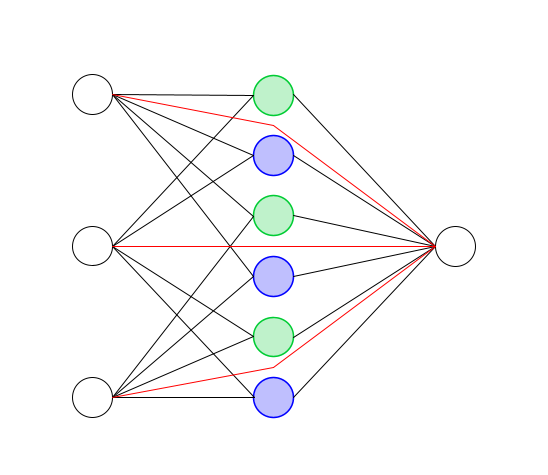
\includegraphics[height=\moyen]{pict/chnet1}
	\caption{Architecture d'un réseau de Choquet}
	\label{fig:chnet1}
    \vspace{-10pt}
    \begin{center}
        \tiny
        \textit{
        En bleu, des neurone de fonction principale $\min(X)$. \\
        En vert, des neurone de fonction principale $\max(X)$.
        }
    \end{center}
\end{figure}
\vspace{-12pt}
Ici, trois problèmes non triviaux se posent (\textit{cf.}\ \ref{subsec:réseau-de-neurones}) :
\begin{itemize}
    \item Les neurones collorées n'appliquent pas une simple application linéaire.
    \item Les neurones ne sont pas reliés en mode Dense mais en convolution.
    \item Certains neurones passent des informations en sautant une couche de neurones.
\end{itemize}


\paragraph{Une autre piste à donc été envisagée :}
Créer un réseau simple comme dans la figure\ \ref{fig:net3}.
Dans ce réseau, aucuns neurone n'a de fonction complexe :
ceux de gauche sont les entrées et
celui de droite fait le produit scalaire avec un vecteur poids.
\begin{figure}[H]
    \center
    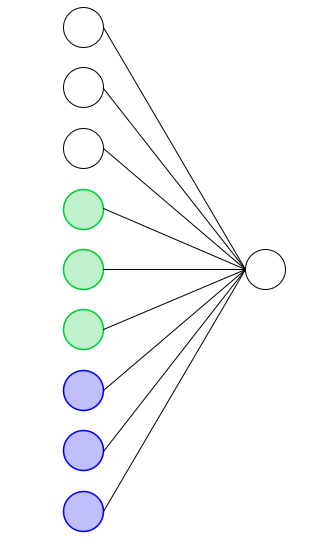
\includegraphics[height=\moyen]{pict/net3.png}
	\caption{Réseau alternatif}
	\label{fig:net3}
\end{figure}
\vspace{-12pt}
Ce réseau est bien plus simple à générer : c'est un réseau \emph{Dense} de taille $9$ en entrée.
Et plus généralement $n^2$ pour un vecteur de taille $n$.


\rbox{Démonstation :}
{
Prenons un vecteur de taille $n$,
Le but est d'énumerer le nombre de neurones utiles a l'équation\ (\ref{eq:Choquet}).
Le résultat est le suivant :
\begin{equation}
    n + \dbinom{n}{2} + \dbinom{n}{2} = n + 2 \times \frac{n(n-1)}{2} = n^2
\end{equation}
}

Il faut donc créer un vecteur d'entrée à partir une base de données d'apprentissage.
Cela se fait simplement en concaténant le vecteur $X$ avec les elements pris deux à deux passés
dans les fonctions min et max.\\


Lors de la descente de gradient, le réseau traite les poids indiférement,
pour les récupérer les poids de l'équation\ (\ref{eq:Choquet})
il sufit de prendre les $n$ premiers pour $W$,
les $\frac{n(n-1)}{2}$ suivant pour $W_m$
et les $\frac{n(n-1)}{2}$ derniers pour $W_M$.


\newpage
\section{Données réelles}\label{sec:données-réelles}
Une base de données disponible en ligne sur \textsc{Kaggle} a aussi été étudiée\cite{kaggle}.
La base de données traite des prix de maisons vendues entre $2014$ et $2015$
dans le King Country, \textsc{wa}, \textsc{usa}.\\


Pour rechercher les fonctions d'utilités, une liste de fonctions possible a été dressée:
\begin{itemize}
    \item Polynomes de degrés allant de $1$ à $3$
    \item Exponentiel
    \item Logarithme
    \item Hyperbolique
    \item Racine
    \item Sigmoide
    \item Gaussienne
\end{itemize}
Une fois toutes ces fonctions codées, chaque plage de données à essayé d'être régressée grâce à celles-ci.
L'efficacité de la regression a été mesurée grâce aux moindres carrés (mean squared error ou $R^2$).
La fonction obtenant le meilleur $R^2$ a été conservé pour chaque pages de données.
Afin de retirer les données n'agissant pas sur le prix,
les fonctions d'utilités présentant un $R^2$ inférieur à $0.3$ ont été retirées.\\


En utilisant les fonctions d'utilités trouvées précédemment, un réseau de Choquet a été créé puis entrainé
sur cette base de données.
L'entrainement est cependant long, environ $8$h sur cluster de calcul du \lri.
Ce temps a pu être réduit grâce à de l'optimisation et de la programmation parallèle.


